\begin{figure}[h]
        \centering
        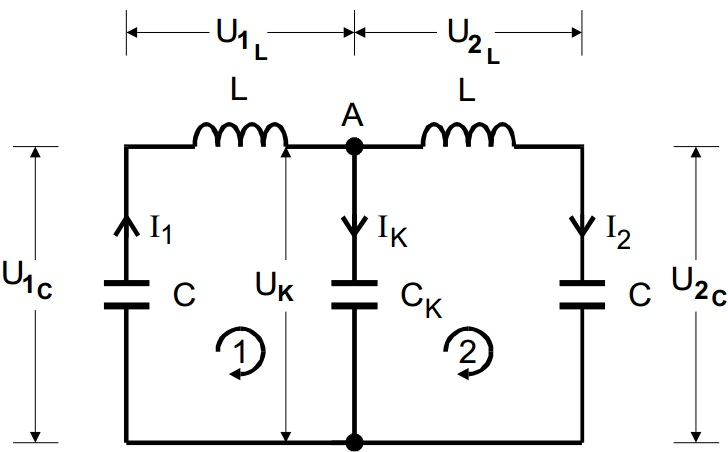
\includegraphics[scale=0.5]{Grafiken/V355Abb1.jpg}
        \caption{Prinzipschaltbild zweier kapazitiv gekoppelter Schwingkreise \cite{V355}}
        \label{fig:Abb1}
\end{figure}
Nach der Kirchhoff'schen Knotenegel gilt der Betrag der in einen Knoten fließenden Ströme entspricht dem, der hinaus fließenden Ströme. (s. Abb.1)
\begin{equation}
I_K = I_1 - I_2
\end{equation}
Für die Maschen aus Abb.2 gilt:
\begin{equation}
U_{1C} + U_{1L} + U_K = 0
\end{equation}
und
\begin{equation}
U_{2C} + U_{2L} + U_K = 0
\end{equation}
Aus diesen Grundsätzlichen Gleichungen lässt sich die Schwingungsfrequenz
\begin{equation}
v^+ = \frac{1}{2 \pi \sqrt{L C}}
\label{eq:f+}
\end{equation}
und die Frequenz
\begin{equation}
v^- = \frac{1}{2 \pi \sqrt{L\left(\frac{1}{C} + \frac{2}{C_K}\right)^{-1}}}
\label{eq:f-}
\end{equation}
bestimmen. \\
Mit Hilfe der Maschenregel und Betrachtung der komplexen Widerstände ergibt sich der Betrag von $I_2$ zu:
\begin{equation}
|\mathfrak{I}_2| = |\mathfrak{U}| \frac{1}{\sqrt{4 \omega^2 C_K^2 R^2 Z(\omega )^2 + \left(\frac{1}{\omega C_K} - \omega C_K Z(\omega )^2 + \omega R^2 C_K\right)}}
\label{eq:I2}
\end{equation}
mit der Vereinfachung:
\begin{equation*}
Z(\omega ) := \omega L - \frac{1}{\omega } \left(\frac{1}{C} + \frac{1}{C_K}\right) 
\end{equation*}
